\chapter{背景}
\label{background}



本章では, 本研究の背景を示す.

\section{自動運転}

車における自動運転は1980年代から研究されてきた.
例えば, 欧州で1987年から1995年に行われたEUREKAプロメテウス計画\footnote[1]{https://www.eurekanetwork.org/project/id/45}では高速道路における車線の追従や車線の変更などの自動運転の基礎技術が研究された.
現在では, これらの機能は市販の自家用車にも運転を支援する機能として搭載されている. また, 高速道路など限定した場所であれば人間による介入が不要な一部自動運転が可能となっているものもある.
今後, 将来自動運転技術はより人間による操作を少なくし, 首相官邸ホームページ「官民 ITS 構想・ロードマップ 2019」\footnote[2]{https://www.kantei.go.jp/jp/singi/it2/kettei/pdf/20190607/siryou9.pdf}に定義されたレベル5の完全な自動運転技術が完成する可能性がある.



\section{Mobility as a Service}

日本に置いて, 車や鉄道などの交通は高度経済成長期以降, 道路網や路線網の拡大も合わせて急速に普及が進み, 旅客・貨物共に主たる移動手段となった. 

しかし, 近年, 交通は単なる移動手段としてだけではなく, 移動や移動に付随する付加価値や自己所有の車を自ら運転すると行った従来の使い方からの変化が求められるようになってきた.

これに対して移動をサービスとして提供するという考え方があり, Mobility as a Serviceの略称MaaSと呼ばれている. 現在MaaSサービスとしては米Uberなどに代表される個人所有の車を配車するサービスや, 自動車を不特定多数の利用者で共有するカーシェアリングサービスなどがある.

人間による操作を必要としないレベル5の自動運転が実現すると, ハンドルを握る必要がないため従来のように自動車において移動時間中に運転に拘束されることがない.
また, 移動経路も人間が考えることなく目的地まで到達する. このようになると, 単に自動車そのものを共有するサービスだけではなく
移動経路の選択や移動時間の活用などのサービスとして提供する事が必要になると予想される.

\section{シェアリングエコノミー}

シェアリングエコノミー\cite{Sharing}ないしは共有経済とはモノやサービスを特定の個人で所有するのではなく複数人で共有する社会関係もしくは社会システムである.
古くはGNUプロジェクトなどのオープンソースソフトウェアがそれに当たると考えられている.
スマートフォンの普及により人々は常時インターネットに接続するようになった, これによりUber\footnote[1]{https://www.uber.com/jp/ja/}などの個人所有の車の配車サービスやAirBnb\footnote[2]{https://www.airbnb.jp}などの所有する不動産を一定期間旅館のような形で貸し出すと行ったサービスが登場し,
社会的に大きな影響をもたらしている.
将来, 人間が介在することのない自動運転が可能になると自動車そのもののハードウェアをシェアするだけではなく自動車を使ったサービスのシェアが加速すると思われる.


\section{機械学習}

機械学習とはコンピューターが自動的にパターンを学習し人間による指示がなくとも課題を実行する事である.
モバイルコンピューターの性能が飛躍的に向上し画像の認識や機械翻訳などの多くの分野で応用されるようになってきた.
これらの技術は日々進化を重ねており画像分類の分野においては1年で認識率を20\%向上したり, 学習にかかる時間を50\%ほど短縮するアルゴリズムが考案されたりと飛躍的に向上してる.
また, 機械学習アルゴリズムは意思決定を伴う処理にも活用され, AlphaGo~\cite{AlphaGo}に代表されるように囲碁などのボードゲーム分野におて人間をも上回る成果を出している.
加えて, 意思決定型の機械学習はボードゲーム意外にも応用されつつあり, リスティング広告の最適化など利用者である人間にとっての利益が最大化するような制御に応用されつつある.





\subsection{機械学習}

機械学習とは広義には, コンピューターが自動的にパターンを学習し人間による明示的な命令がなくとも
特定の課題を自動で実行する技術又はアルゴリズムのことである. 主に, 正解データを与えることによってパターンを学習する教師あり学習,
データのまとまりや相関を求める教師なし学習と繰り返し反復することで価値が最大化するように学習を行う強化学習に分類される.
画像処理や自然言語処理など様々な分野に応用が進んでおり, 画像の検知や自動翻訳など機械学習によって自動化されているものも多い.


\subsection{深層学習}

深層学習とは脳が持つ脳神経系のニューロンをソフトウェアで再現した人工ニューラルネット(ANN)を持つ機械学習アルゴリズムの一つである. 
人間の脳を模したパーセプトロン~\cite{Perceptron}による深層学習自体は1957年から提唱されていた. しかし, 4層以上のパーセプトロンでは過学習や勾配消失問題が発生しやすく計算コストも大きいためあまり普及しなかった.
しかし, 安価なコンピューターでも計算速度が飛躍的に向上したことや勾配消失問題を防止する手法が考案されたことなどから再び注目を集めるようになり, 様々な課題に特価したDNNが考案されている.

例えば, Convolutional Neural Network (CNN)~\cite{CNN}は画像の特徴量抽出に長けており画像認識分野で大きな成果をあげている.
Long short-term memory (LSTM) ~\cite{LSTM}は自動翻訳やテキスト解析など自然言語処理分野で活用されており, 現在では言語だけではなく音楽などにも活用範囲が広がっている.
また, 既存の機械学習の手法に深層学習を組み込んだ事例も散見される.

\subsection{多層パーセプトロン}
パーセプトロンとは


\begin{figure}[H]
    \centering
    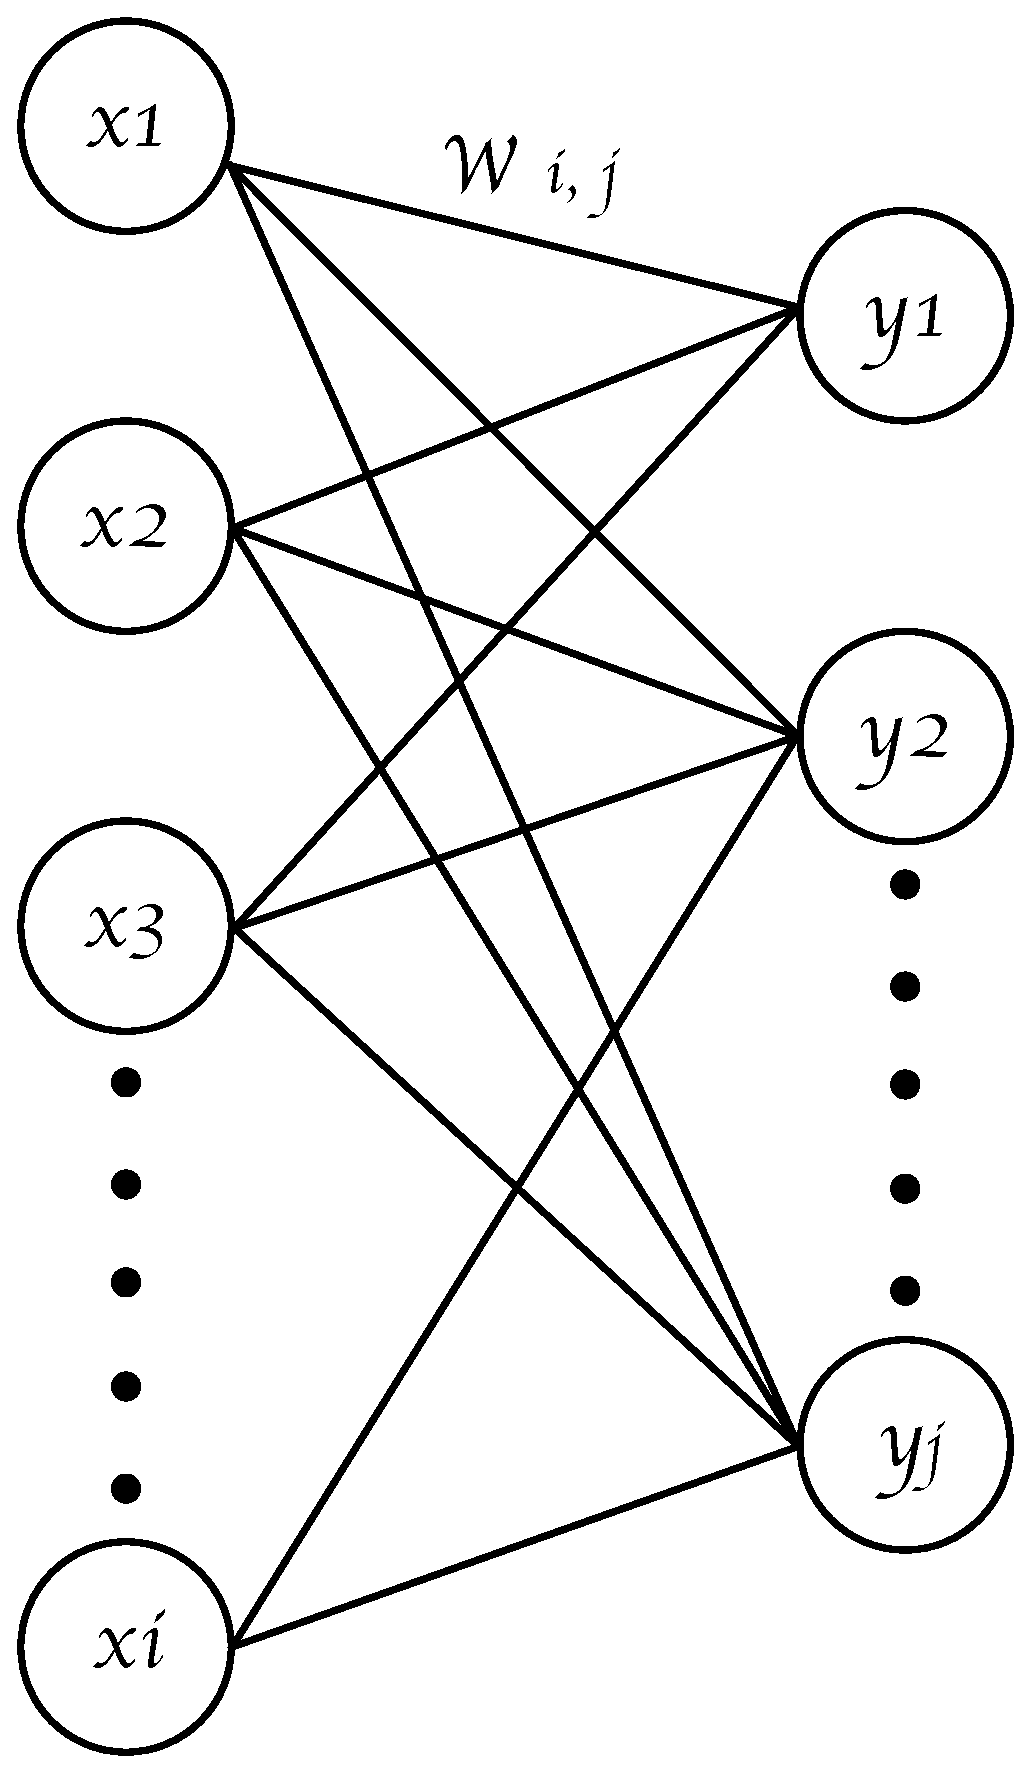
\includegraphics[clip,height = 8.0cm]{assets/perceptron.eps}
    \caption{パーセプトロン}  \label{sample}
\end{figure}

\subsection{強化学習}

強化学習 (Reinforcement learning) ~\cite{ReinforcementLearning}はエージェントと呼ばれる行動主体が現在の状態を観測し価値が最大化する行動を繰り返し選択することにより利益が最大になる行動を学習する機械学習手法の一種である.
強化学習では行動主体であるエージェントと環境を定義する状態と行動した結果による変化, 報酬が定義される.
初期的な強化学習にはマルコフ決定過程~\cite{ReinforcementLearning}やQ学習~\cite{QL}というものがある.

\subsection{深層強化学習}

深層強化学習とは, 強化学習に深層学習を組み合わせた機械学習アルゴリズムである.
強化学習はエージェントとエージェントが動作する環境を定義し, 定義された環境下でエージェントへの報酬が最大化するように学習は行う.

\begin{figure}[H]
    \centering
    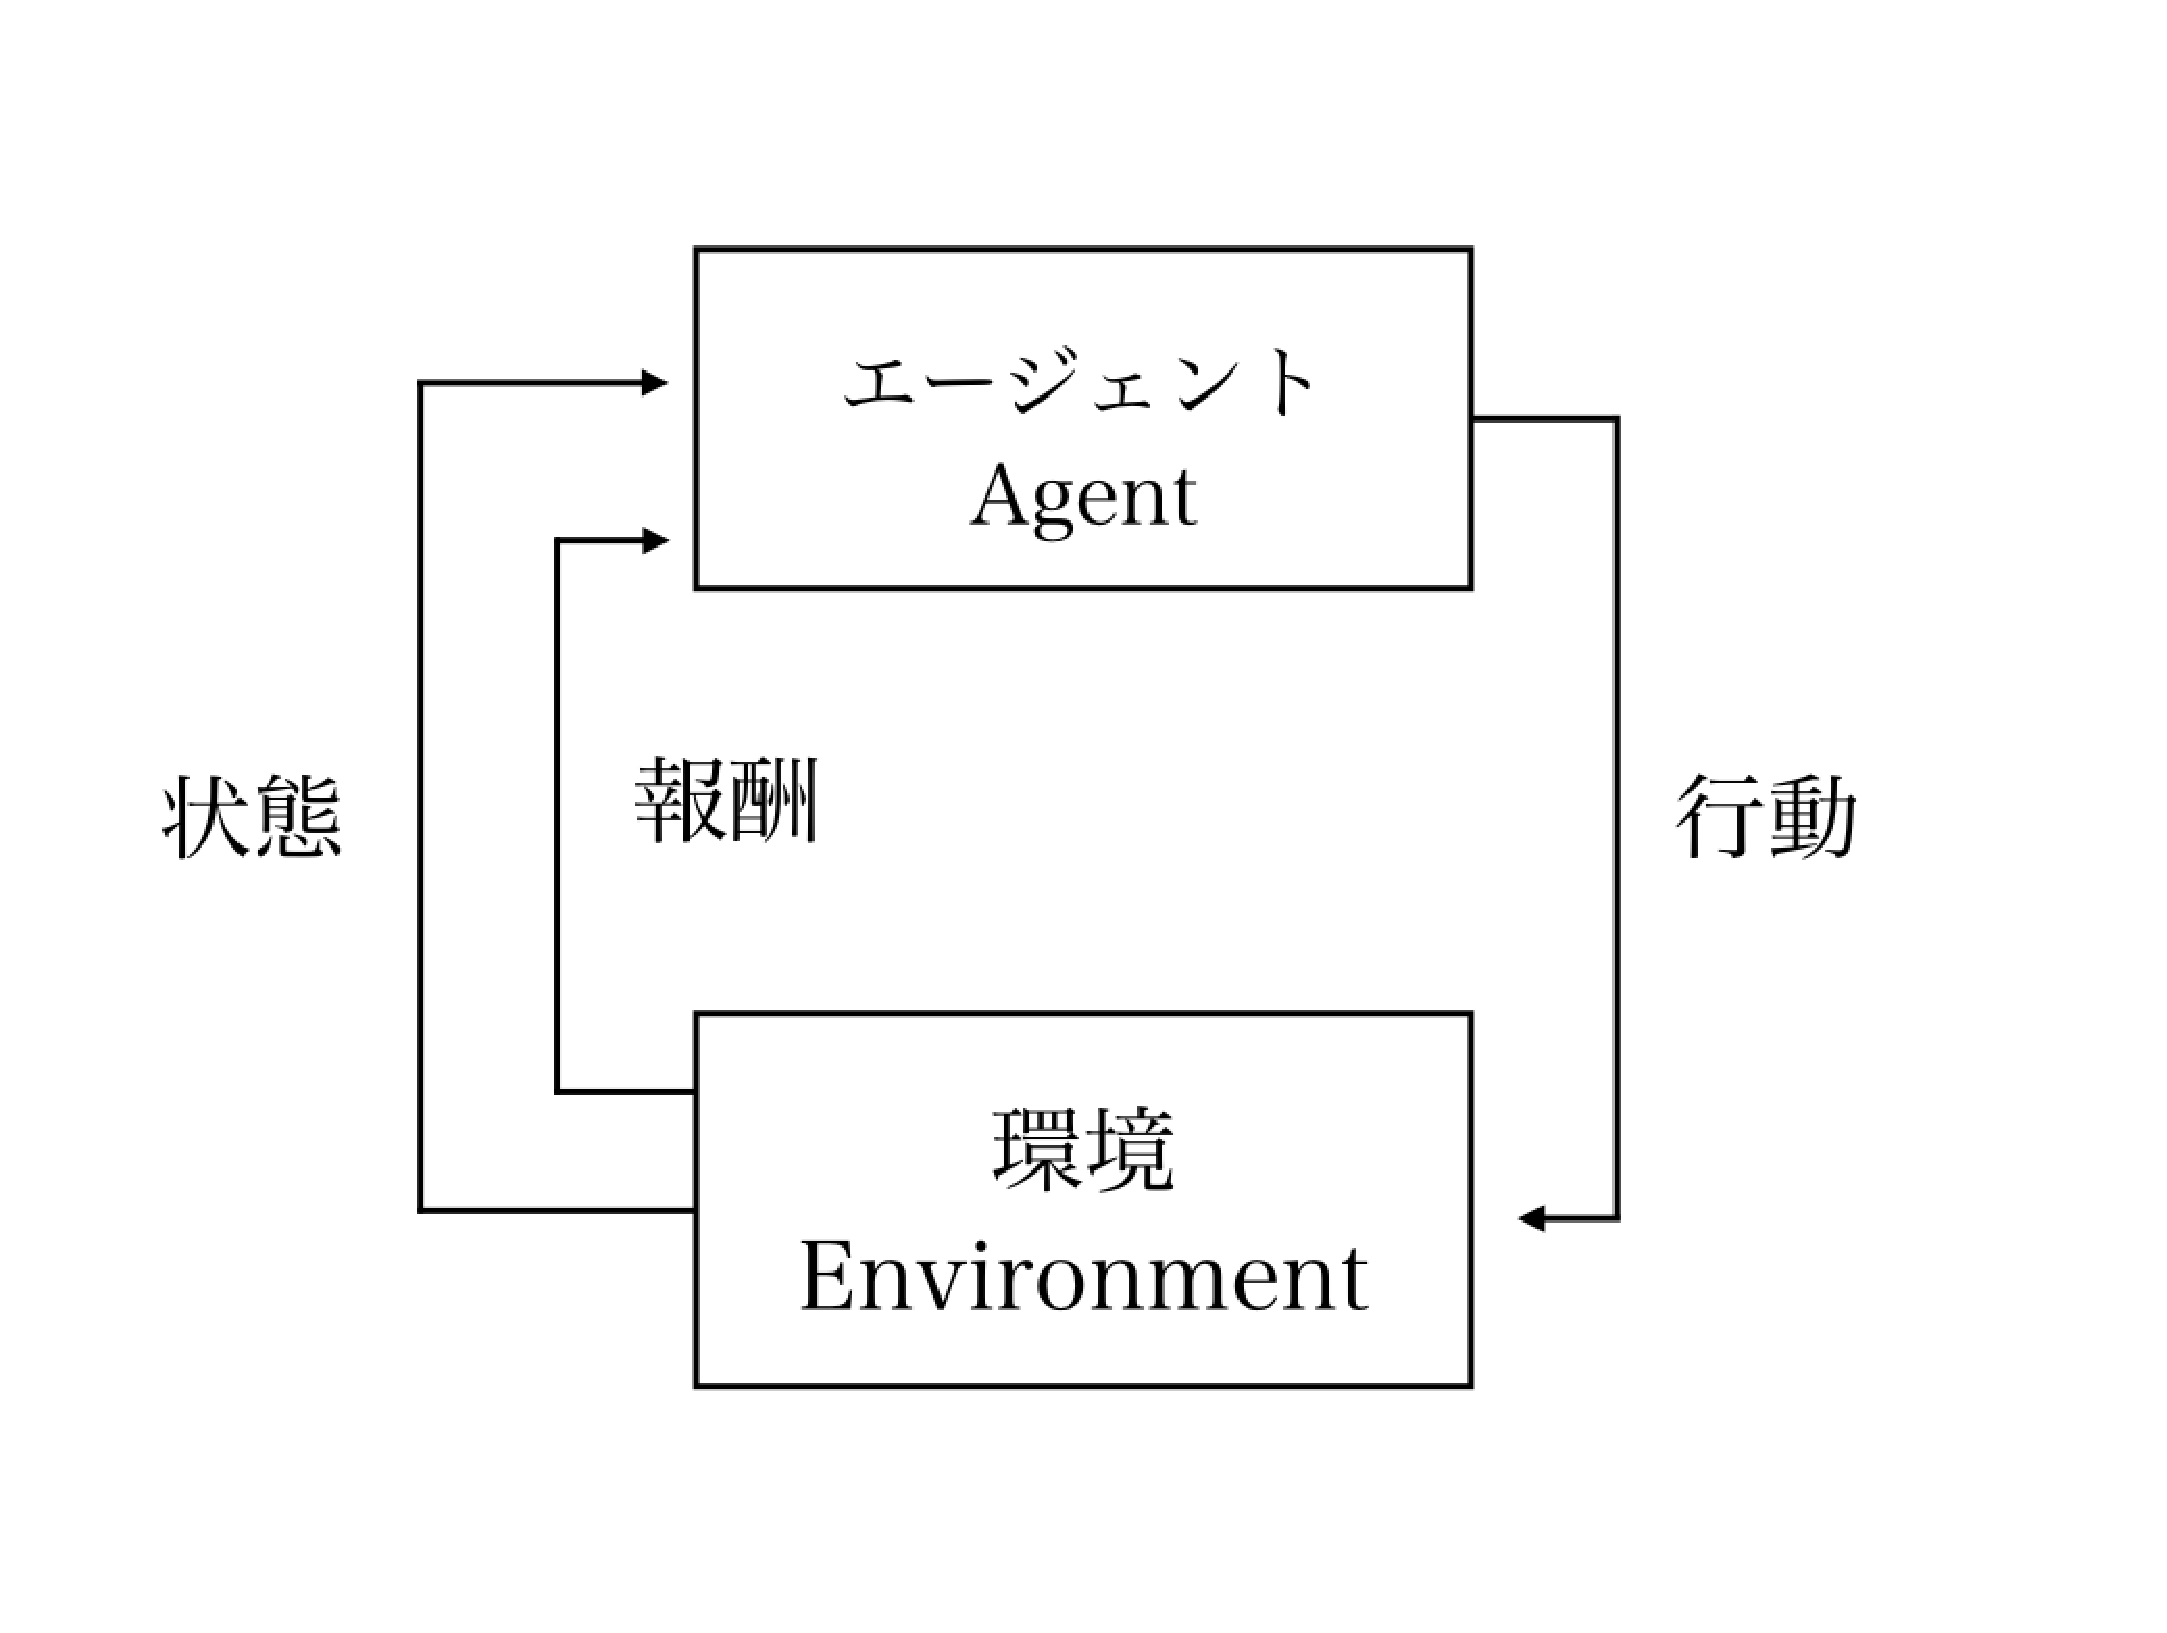
\includegraphics[clip,width = 12.0cm]{assets/reinforcement_learning.eps}
    \caption{強化学習の概念図}  \label{sample}
\end{figure}

\section{Q学習}

Q学習とは初期に考案されたReinforest Learningアルゴリズムの一種であり, 強化学習と呼ばれす.
Q学習による試行は以下のように定義する.

\begin{equation}
    Q(s, a) \approx R(s, a) + \gamma max_{a'} E[Q(s', a')]
\end{equation}

\section{Deep Q Neural Network}

Deep Q Neural Network(DQN~\cite{DQN})の一種でQ学習という強化学習における古典的なアルゴリズムを深層強化学習に応用したものである.
\textcolor{red}{ちょと再考}
Q学習~\cite{QL}とは強化学習の一種である. Q学習~\cite{QL}では実行するルールに対してQ値という値を持たせる.

DQNの深層学習部分はCNN~\cite{DQN}で構成される.

\begin{figure}[H]
    \centering
    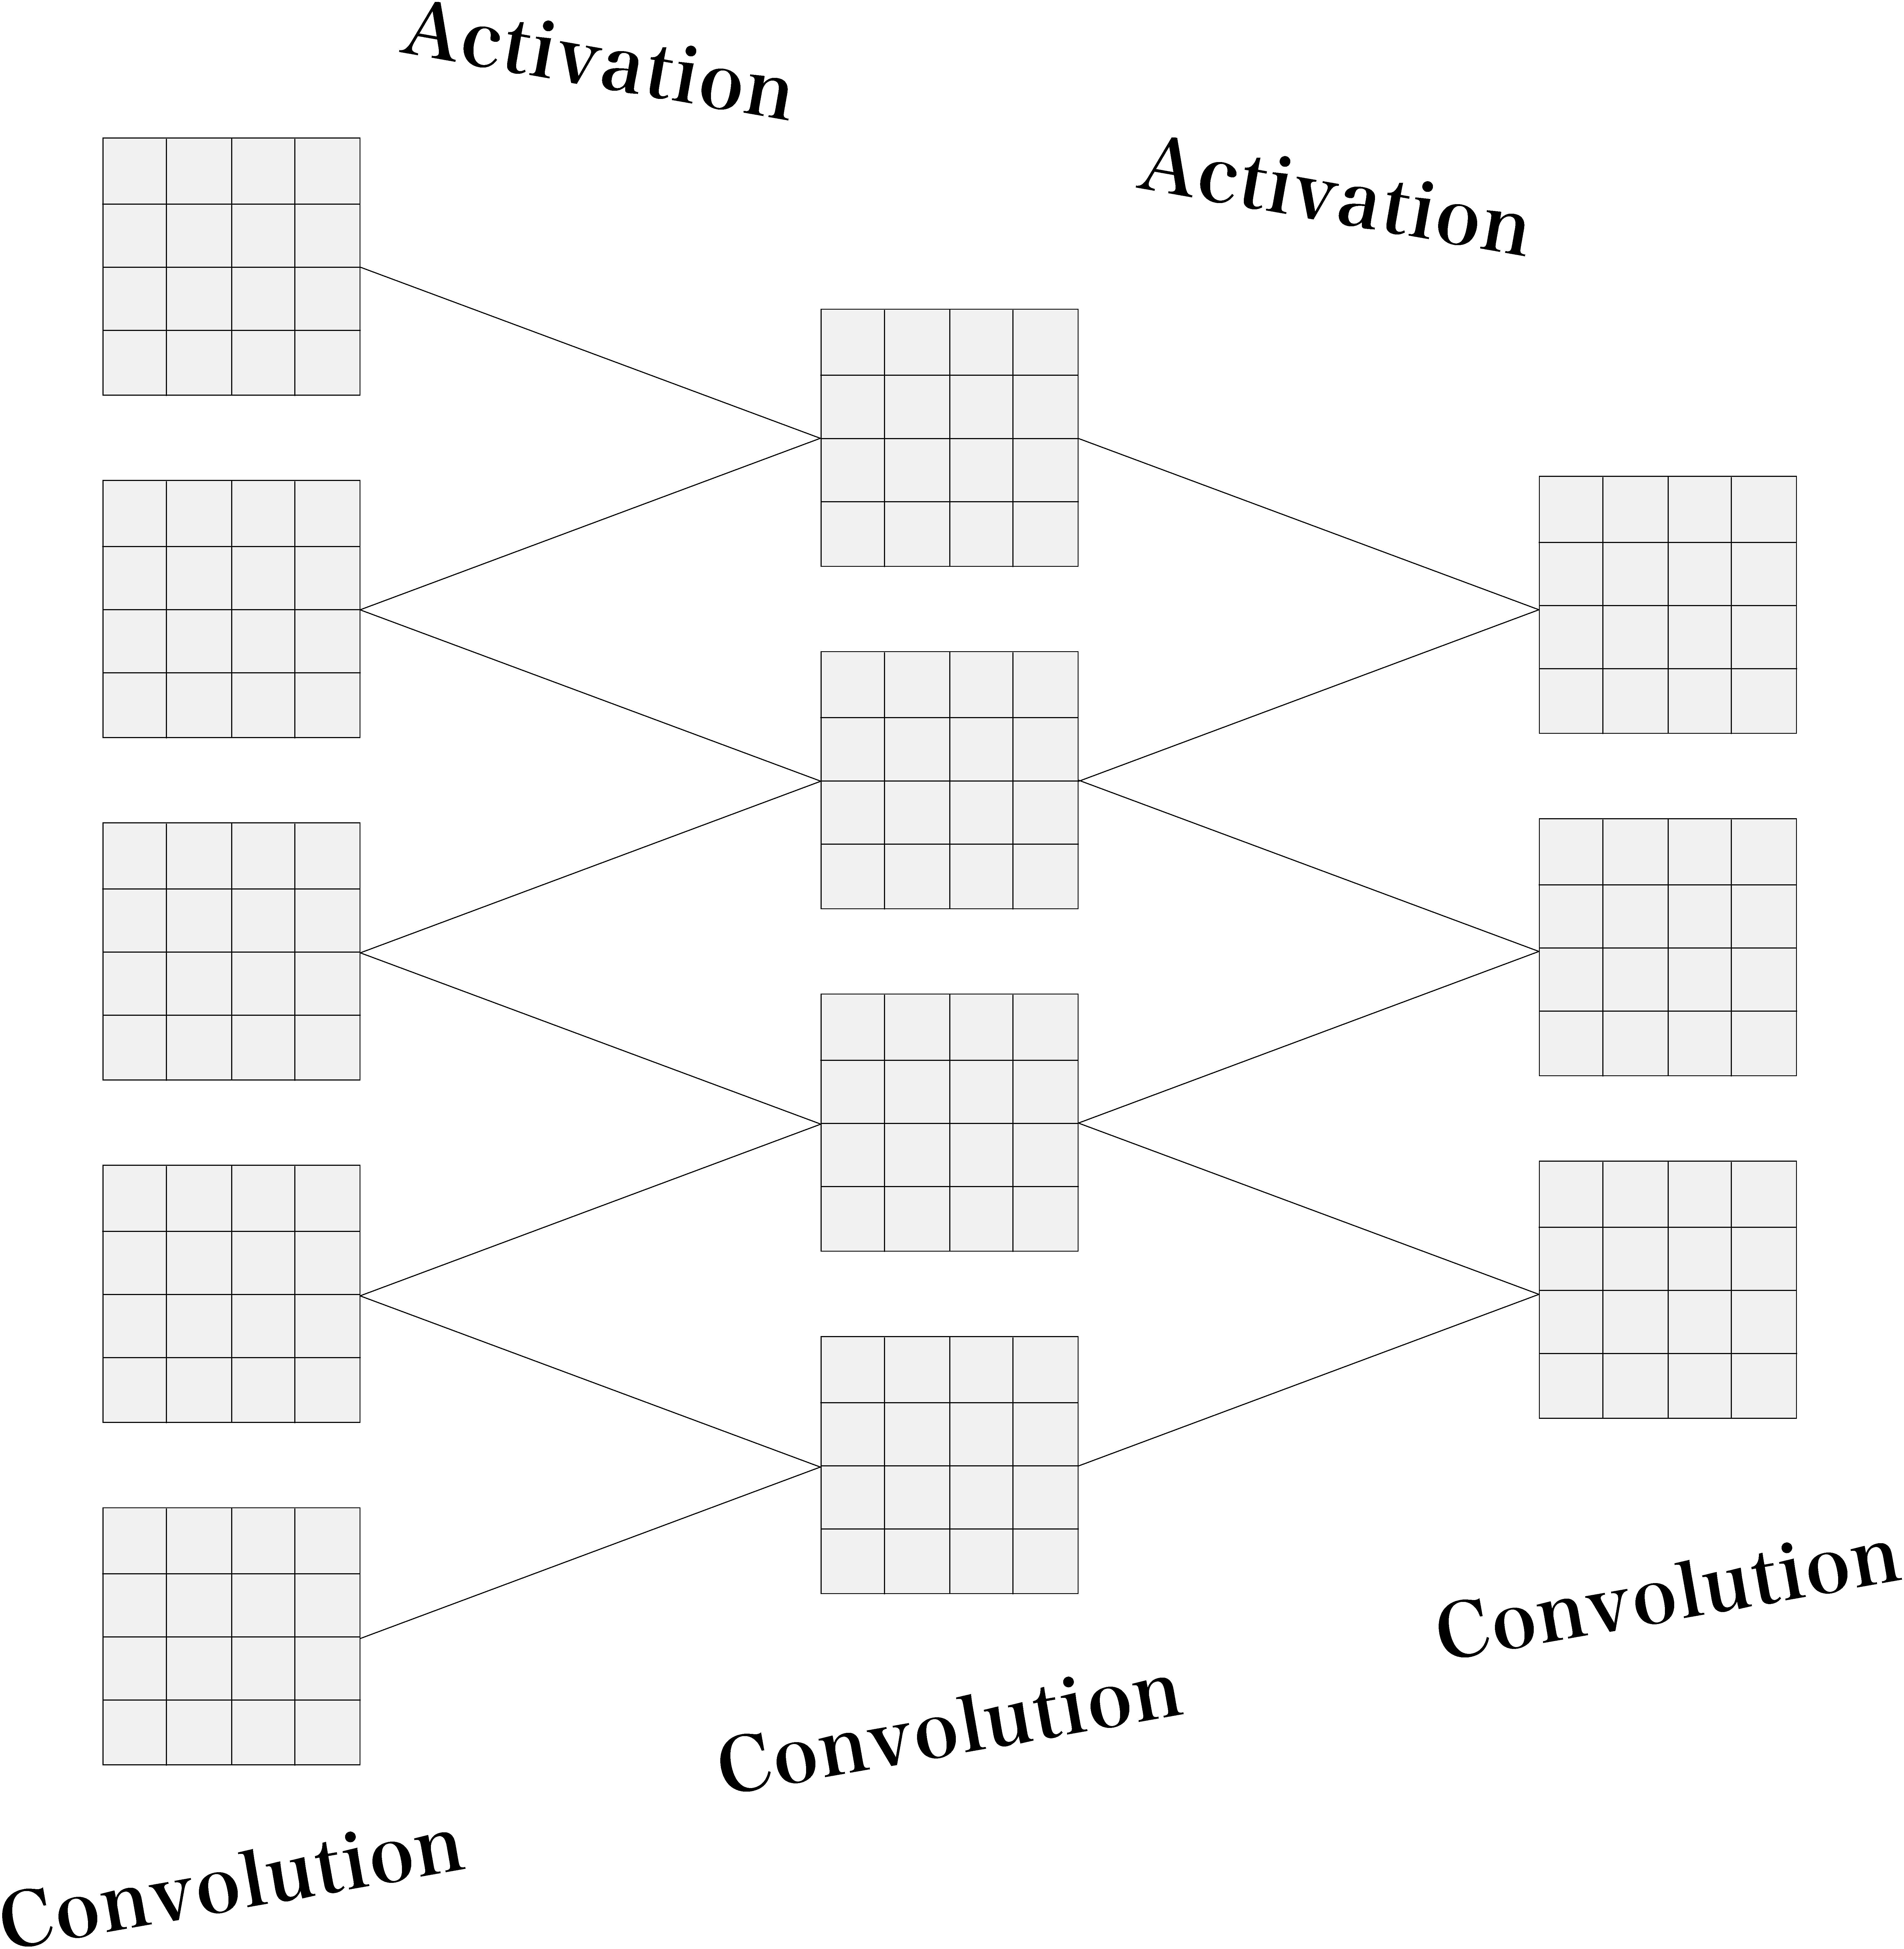
\includegraphics[clip,height = 8.0cm]{assets/dqn_convolution.eps}
    \caption{DQNを構成するCNN}  \label{sample}
\end{figure}




\begin{figure}[H]
    \centering
    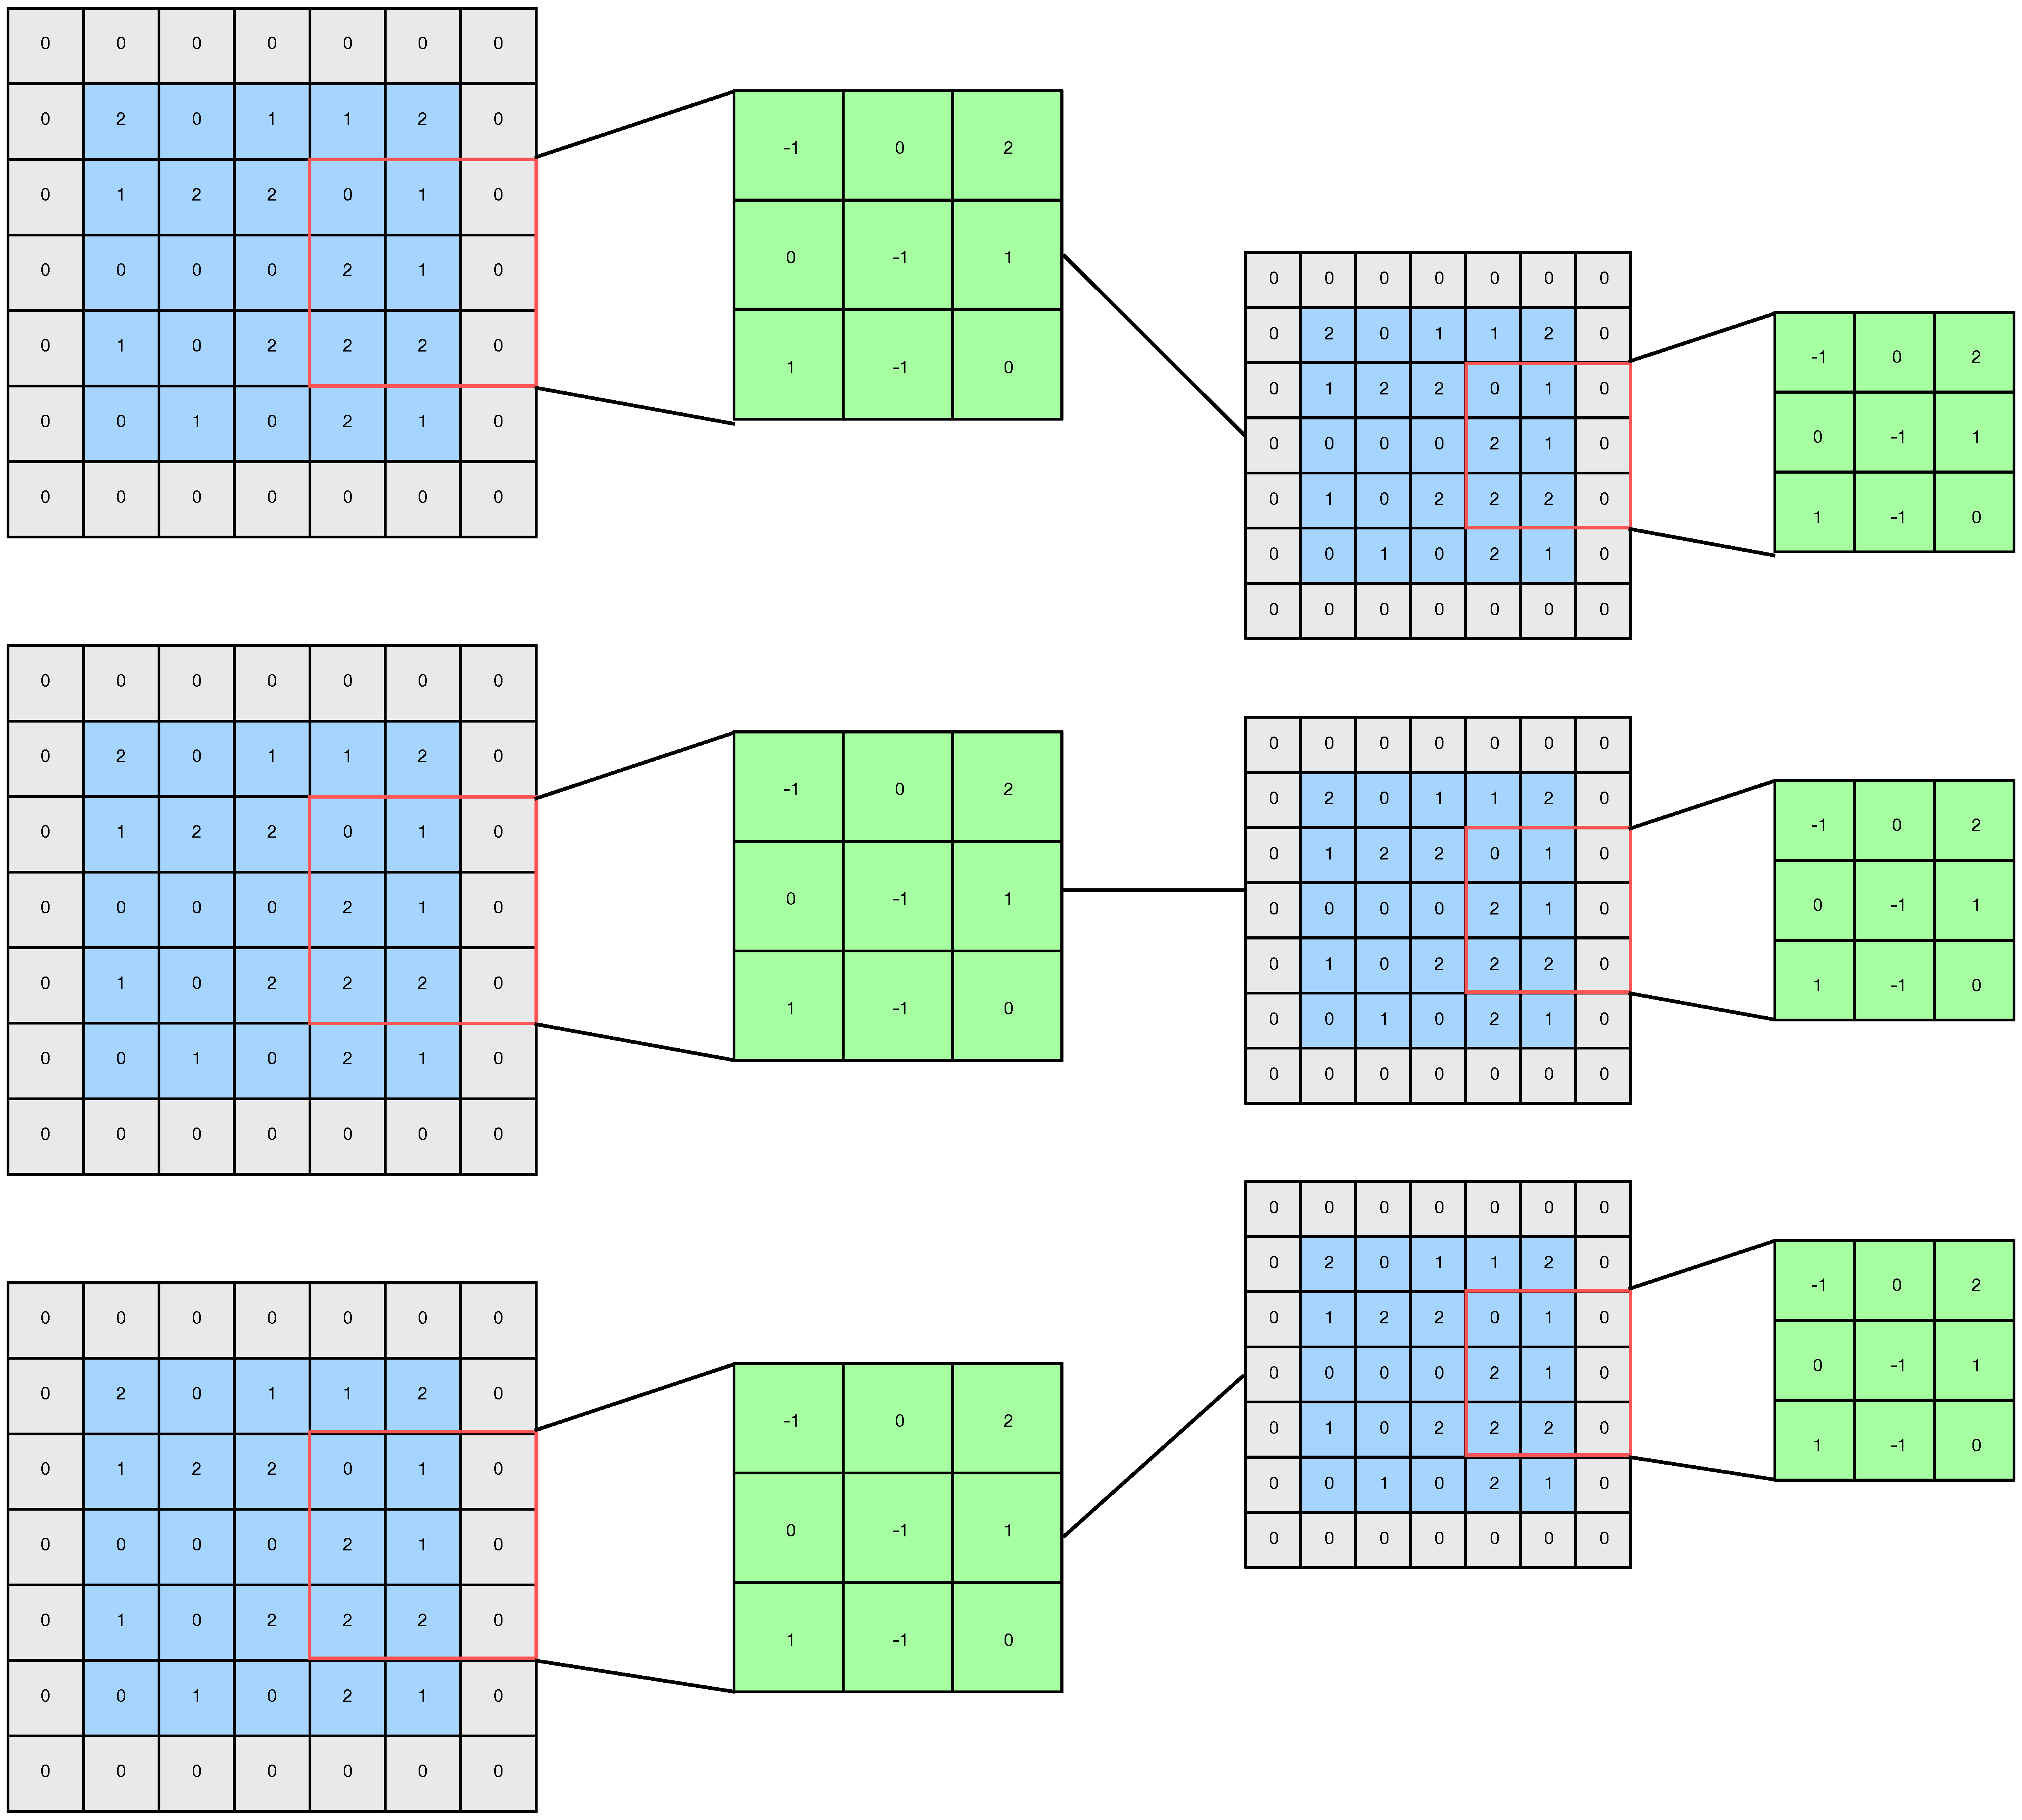
\includegraphics[clip,height = 8.0cm]{assets/CNN_typical.eps}
    \caption{一般的なConvolutional Neural Network}  \label{sample}
\end{figure}



%%% Local Variables:
%%% mode: japanese-latex
%%% TeX-master: "../thesis"
%%% End:
